%%%%%%%%%%%%%%%%%%%%%%%%%%%%%%%%%%%%%%%%%%%%%%%%%%%%%%%%%%%%%%%%%%%%%%%%%%%%%%%%
%2345678901234567890123456789012345678901234567890123456789012345678901234567890
%        1         2         3         4         5         6         7         8
%% PP_Report.tex
%% V1.4
%% 2015/11/30
%% by Rui Santos Cruz
%% This is a skeleton file using PPIEEEtran.cls
%% (requires PPIEEEtran.cls) 
% !TEX root = ./main.tex
%%%%%%%%%%%%%%%%%%%%%%%%%%%%%%%%%%%%%%%%%%%%%%%%%%%%%%%%%%%%%%%%%%%%%%%%%%%%%%%%
\documentclass[a4paper,12pt,journal,twoside,compsoc]{PPIEEEtran}

% -----------------------------------------------------------------------------
% The Preamble document contains all the necessary Packages for typesetting
% Modify it to suit your needs
% -----------------------------------------------------------------------------
%%%%%%%%%%%%%%%%%%%%%%%%%%%%%%%%%%%%%%%%%%%%%%%%%%%%%%%%%%%%%%%%%%%%%%%%%%%%%%%%
%2345678901234567890123456789012345678901234567890123456789012345678901234567890
%        1         2         3         4         5         6         7         8
% Required Packages and commands
% --> Please Choose the MAIN LANGUAGE for the document in package BABEL (below)
% --> Please Choose the TYPE OF REPORT for the document in \ReportType (below)
% !TEX root = ./main.tex
% PP_Report_Preamble.tex
% V1.4
% 2015/11/30
% by Rui Santos Cruz
%%%%%%%%%%%%%%%%%%%%%%%%%%%%%%%%%%%%%%%%%%%%%%%%%%%%%%%%%%%%%%%%%%%%%%%%%%%%%%%%
%
% *** INPUT LANGUAGE PACKAGES ***

\usepackage[main=english]{babel}
\usepackage[utf8]{inputenc}
\usepackage{iflang}

% *** DEFINE THE TYPE OF REPORT ***
\newcommand*{\ReportType}{learning}% Uncomment line for Learning Report
%\newcommand*{\ReportType}{activity}% Uncomment line for Activity Report

% *** ACRONYM PACKAGES ***
% Put definition of Acronyms at the end of the document
\usepackage[printonlyused,nolist]{acronym}

% *** CITATION PACKAGES ***
\usepackage{cite}

% *** GRAPHICS RELATED PACKAGES ***
\usepackage[pdftex]{graphicx}
\DeclareGraphicsExtensions{.pdf,.jpeg,.png}

% *** MATH PACKAGES ***
\usepackage[cmex10]{amsmath}

% *** SPECIALIZED LIST PACKAGES ***
\usepackage{algorithmic}

% *** ALIGNMENT PACKAGES ***
\usepackage{array}

% *** SUBFIGURE PACKAGES ***
\usepackage[caption=false,font=normalsize,labelfont=sf,textfont=sf]{subfig}

% *** FLOAT PACKAGES ***
\usepackage{fixltx2e}

% *** PDF, URL AND HYPERLINK PACKAGES ***
\usepackage{url}

% *** BACKGROUND Material ***
\usepackage{eso-pic}
\usepackage[
  contents={},
  opacity=1,
  scale=1,
  color=blue!90
  ]{background}
  
% *** CONDITIONALS ***
\usepackage{ifthen}

% DEFINE COMMAND FOR: Report Type depending on language
\newcommand{\tlangRepActivity}{\IfLanguageName{english}{Activity Report}{Relatório de Atividade}}
\newcommand{\tlangRepLearning}{\IfLanguageName{english}{Learnings Report}{Relatório de Aprendizagens}}
%%%%%%%%%%%%%%%%%%%%%%%%%%%%%%%%%%%%%%%%%%%%%%%%%%%%%%%%%%%%%%%%%%%%%%%%%%%%%%%%
% DEFINE COMMAND FOR: Report Scoring Table Type
\newcommand{\lrScore}%
{\setlength{\unitlength}{1mm}{% % selecting unit length 
\fontfamily{phv}\selectfont
\begin{picture}(171.6,20) % picture environment with the size (dimensions)
% 32 length units wide, and 15 units high.
\setlength\fboxsep{0pt}
% Left Set with grading Scores
\put(0,0){\fcolorbox{gray}{gray!20}{%
          \framebox(15,4)[l]{\scriptsize{0.2-Weak}}}}
\put(0,4){\fcolorbox{gray}{gray!20}{%
          \framebox(15,4)[l]{\scriptsize{0.4-Fair}}}}
\put(0,8){\fcolorbox{gray}{gray!20}{%
          \framebox(15,4)[l]{\scriptsize{0.6-Good}}}}
\put(0,12){\fcolorbox{gray}{gray!20}{%
           \framebox(15,4)[l]{\scriptsize{0.8-V.Good}}}}
\put(0,16){\fcolorbox{gray}{gray!20}{%
           \framebox(15,4)[l]{\scriptsize{1.0-Excel}}}}
% Left+1 Set with Learning Rubrics
\put(16,0){\fcolorbox{cyan}{white}{%
          \framebox(12,12)[c]{\footnotesize{ }}}}
\put(28,0){\fcolorbox{cyan}{white}{%
          \framebox(12,12)[c]{\footnotesize{ }}}}          
\put(40,0){\fcolorbox{cyan}{white}{%
          \framebox(12,12)[c]{\footnotesize{ }}}}
\put(52,0){\fcolorbox{cyan}{white}{%
          \framebox(12,12)[c]{\footnotesize{ }}}}
\put(64,0){\fcolorbox{cyan}{white}{%
          \framebox(12,12)[c]{\footnotesize{ }}}}
\put(16,12){\fcolorbox{cyan}{white}{%
          \framebox(12,4)[c]{\tiny{Intro$\times 2$}}}}
\put(28,12){\fcolorbox{cyan}{white}{%
          \framebox(12,4)[c]{\tiny{Motiv$\times 2$}}}}          
\put(40,12){\fcolorbox{cyan}{white}{%
          \framebox(12,4)[c]{\tiny{Skills$\times 6$}}}}
\put(52,12){\fcolorbox{cyan}{white}{%
          \framebox(12,4)[c]{\tiny{Reflect$\times 6$}}}}
\put(64,12){\fcolorbox{cyan}{white}{%
          \framebox(12,4)[c]{\tiny{Sugg$\times 2$}}}}
\put(16,16){\fcolorbox{cyan}{cyan!20}{%
          \framebox(60,4)[c]{\footnotesize{LEARNINGS}}}}
% Middle Set with Document Rubrics
\put(77,0){\fcolorbox{green}{white}{%
          \framebox(12,12)[c]{\footnotesize{ }}}}
\put(89,0){\fcolorbox{green}{white}{%
          \framebox(12,12)[c]{\footnotesize{ }}}}
\put(101,0){\fcolorbox{green}{white}{%
          \framebox(12,12)[c]{\footnotesize{ }}}}
\put(113,0){\fcolorbox{green}{white}{%
          \framebox(12,12)[c]{\footnotesize{ }}}}
\put(125,0){\fcolorbox{green}{white}{%
          \framebox(12,12)[c]{\footnotesize{ }}}}
\put(137,0){\fcolorbox{green}{white}{%
          \framebox(12,12)[c]{\footnotesize{ }}}}
\put(77,12){\fcolorbox{green}{white}{%
          \framebox(12,4)[c]{\tiny{Struct $\times .25$}}}}
\put(89,12){\fcolorbox{green}{white}{%
          \framebox(12,4)[c]{\tiny{Ortog$\times .25$}}}}          
\put(101,12){\fcolorbox{green}{white}{%
          \framebox(12,4)[c]{\tiny{Gram$\times .25$}}}}
\put(113,12){\fcolorbox{green}{white}{%
          \framebox(12,4)[c]{\tiny{Form $\times .25$}}}}
\put(125,12){\fcolorbox{green}{white}{%
          \framebox(12,4)[c]{\tiny{Abstr $\times .5$}}}}
\put(137,12){\fcolorbox{green}{white}{%
          \framebox(12,4)[c]{\tiny{Concl $\times .5$}}}}
\put(77,16){\fcolorbox{green}{green!20}{%
          \framebox(72,4)[c]{\footnotesize{DOCUMENT}}}}
% Right Set with Penalties
\put(150,0){\fcolorbox{red}{white}{%
          \framebox(10,12)[c]{\footnotesize{ }}}}
\put(160,0){\fcolorbox{red}{white}{%
          \framebox(10,12)[c]{\footnotesize{ }}}}
\put(170,0){\fcolorbox{red}{white}{%
          \framebox(10,12)[c]{\footnotesize{ }}}}
\put(150,12){\fcolorbox{red}{white}{%
          \framebox(10,4)[c]{\tiny{Titles $\times .5$}}}}
\put(160,12){\fcolorbox{red}{white}{%
          \framebox(10,4)[c]{\tiny{Files $\times .5$}}}}
\put(170,12){\fcolorbox{red}{white}{%
          \framebox(10,4)[c]{\tiny{IDs $\times .5$}}}}
\put(150,16){\fcolorbox{red}{red!20}{%
          \framebox(30,4)[c]{\footnotesize{PENALTY}}}}
\end{picture}
}}
%%%%%%%%%%%%%%%%%%%%%%%%%%%%%%%%%%%%%%%%%%%%%%%%%%%%%%%%%%%%%%%%%%%%%%%%%%%%%%%%
%\newcommand{\arScore}%
\newcommand{\arScore}%
{\setlength{\unitlength}{1mm}{% % selecting unit length 
\fontfamily{phv}\selectfont
\begin{picture}(171.6,20) % picture environment with the size (dimensions)
% 32 length units wide, and 15 units high.
\setlength\fboxsep{0pt}
% Left Set with grading Scores
\put(0,0){\fcolorbox{gray}{gray!20}{%
          \framebox(15,4)[l]{\scriptsize{0.2-Weak}}}}
\put(0,4){\fcolorbox{gray}{gray!20}{%
          \framebox(15,4)[l]{\scriptsize{0.4-Fair}}}}
\put(0,8){\fcolorbox{gray}{gray!20}{%
          \framebox(15,4)[l]{\scriptsize{0.6-Good}}}}
\put(0,12){\fcolorbox{gray}{gray!20}{%
           \framebox(15,4)[l]{\scriptsize{0.8-V.Good}}}}
\put(0,16){\fcolorbox{gray}{gray!20}{%
           \framebox(15,4)[l]{\scriptsize{1.0-Excel}}}}
% Left+1 Set with Activity Rubrics
\put(16,0){\fcolorbox{yellow}{white}{%
          \framebox(12,12)[c]{\footnotesize{ }}}}
\put(28,0){\fcolorbox{yellow}{white}{%
          \framebox(12,12)[c]{\footnotesize{ }}}}          
\put(40,0){\fcolorbox{yellow}{white}{%
          \framebox(12,12)[c]{\footnotesize{ }}}}
\put(52,0){\fcolorbox{yellow}{white}{%
          \framebox(12,12)[c]{\footnotesize{ }}}}
\put(64,0){\fcolorbox{yellow}{white}{%
          \framebox(12,12)[c]{\footnotesize{ }}}}
\put(16,12){\fcolorbox{yellow}{white}{%
          \framebox(12,4)[c]{\tiny{Intro$\times 2$}}}}
\put(28,12){\fcolorbox{yellow}{white}{%
          \framebox(12,4)[c]{\tiny{Object$\times 2$}}}}          
\put(40,12){\fcolorbox{yellow}{white}{%
          \framebox(12,4)[c]{\tiny{Plan$\times 4$}}}}
\put(52,12){\fcolorbox{yellow}{white}{%
          \framebox(12,4)[c]{\tiny{Exec$\times 6$}}}}
\put(64,12){\fcolorbox{yellow}{white}{%
          \framebox(12,4)[c]{\tiny{Result$\times 4$}}}}
\put(16,16){\fcolorbox{yellow}{yellow!20}{%
          \framebox(60,4)[c]{\footnotesize{ACTIVITY}}}}
% Middle Set with Document Rubrics
\put(77,0){\fcolorbox{green}{white}{%
          \framebox(12,12)[c]{\footnotesize{ }}}}
\put(89,0){\fcolorbox{green}{white}{%
          \framebox(12,12)[c]{\footnotesize{ }}}}
\put(101,0){\fcolorbox{green}{white}{%
          \framebox(12,12)[c]{\footnotesize{ }}}}
\put(113,0){\fcolorbox{green}{white}{%
          \framebox(12,12)[c]{\footnotesize{ }}}}
\put(125,0){\fcolorbox{green}{white}{%
          \framebox(12,12)[c]{\footnotesize{ }}}}
\put(137,0){\fcolorbox{green}{white}{%
          \framebox(12,12)[c]{\footnotesize{ }}}}
\put(77,12){\fcolorbox{green}{white}{%
          \framebox(12,4)[c]{\tiny{Struct $\times .25$}}}}
\put(89,12){\fcolorbox{green}{white}{%
          \framebox(12,4)[c]{\tiny{Ortog$\times .25$}}}}          
\put(101,12){\fcolorbox{green}{white}{%
          \framebox(12,4)[c]{\tiny{Gram$\times .25$}}}}
\put(113,12){\fcolorbox{green}{white}{%
          \framebox(12,4)[c]{\tiny{Form $\times .25$}}}}
\put(125,12){\fcolorbox{green}{white}{%
          \framebox(12,4)[c]{\tiny{Abstr $\times .5$}}}}
\put(137,12){\fcolorbox{green}{white}{%
          \framebox(12,4)[c]{\tiny{Concl $\times .5$}}}}
\put(77,16){\fcolorbox{green}{green!20}{%
          \framebox(72,4)[c]{\footnotesize{DOCUMENT}}}}
% Right Set with Penalties
\put(150,0){\fcolorbox{red}{white}{%
          \framebox(10,12)[c]{\footnotesize{ }}}}
\put(160,0){\fcolorbox{red}{white}{%
          \framebox(10,12)[c]{\footnotesize{ }}}}
\put(170,0){\fcolorbox{red}{white}{%
          \framebox(10,12)[c]{\footnotesize{ }}}}
\put(150,12){\fcolorbox{red}{white}{%
          \framebox(10,4)[c]{\tiny{Titles $\times .5$}}}}
\put(160,12){\fcolorbox{red}{white}{%
          \framebox(10,4)[c]{\tiny{Files $\times .5$}}}}
\put(170,12){\fcolorbox{red}{white}{%
          \framebox(10,4)[c]{\tiny{IDs $\times .5$}}}}
\put(150,16){\fcolorbox{red}{red!20}{%
          \framebox(30,4)[c]{\footnotesize{PENALTY}}}}
\end{picture}
}}

% DEFINE COMMAND FOR: Printing Scoring Table Type
\newcommand\BackgroundPic{%
\put(-15,12){%
\parbox[b][\paperheight]{\paperwidth}{%
\vfill
\centering
\ifthenelse{\equal{\ReportType}{activity}}{\arScore}{\lrScore}}}}
% Printing the Scoring Table
\AddToShipoutPicture*{\BackgroundPic}

% Print Vertical Identifications on even and odd pages
\AddEverypageHook{%
  \ifthenelse{\isodd{\value{page}}}%
  {\backgroundsetup{
    angle=90,
    position={-0.1\textwidth,-1.055\textheight},
    contents={\tiny{PP-2015 V1.4}}
    }% Odd Pages
  }%
  {\backgroundsetup{
    angle=90,
    position={0.97\textwidth,-1.05\textheight},%
    contents={\ifthenelse{\equal{\ReportType}{activity}}{%
              \tiny{\tlangRepActivity}}{\tiny{\tlangRepLearning}}}
    }% Even Pages
  }%
  \BgMaterial}
% correct bad hyphenation here
\hyphenation{op-tical net-works semi-conduc-tor}
%%%%%%%%%%%%%%%%%%%%%%%%%%%%%%%%%%%%%%%%%%%%%%%%%%%%%%%%%%%%%%%%%%%%%%%%%%%%%%%%
%2345678901234567890123456789012345678901234567890123456789012345678901234567890
%        1         2         3         4         5         6         7         8
\begin{document}
%%%%%%%%%%%%%%%%%%%%%%%%%%%%%%%%%%%%%%%%%%%%%%%%%%%%%%%%%%%%%%%%%%%%%%%%%%%%%%%%
%2345678901234567890123456789012345678901234567890123456789012345678901234567890
%        1         2         3         4         5         6         7         8
%% PP_Report_Cover.tex
%% V1.4
%% 2015/11/30
%% by Rui Santos Cruz
% !TEX root = ./main.tex
%%%%%%%%%%%%%%%%%%%%%%%%%%%%%%%%%%%%%%%%%%%%%%%%%%%%%%%%%%%%%%%%%%%%%%%%%%%%%%%%
% paper title
% can use linebreaks \\ within to get better formatting as desired
% Do not put math or special symbols in the title.
\title{Por2folios Platform}
%%%%%%%%%%%%%%%%%%%%%%%%%%%%%%%%%%%%%%%%%%%%%%%%%%%%%%%%%%%%%%%%%%%%%%%%%%%%%%%%
% Author names
%
% note positions of commas and nonbreaking spaces ( ~ ) LaTeX will not break
% a structure at a ~ so this keeps an author's name from being broken across
% two lines.
% use \thanks{} to gain access to the first footnote area
% a separate \thanks must be used for each paragraph.
%
%\IEEEcompsocitemizethanks is a special \thanks that produces the bulleted
% lists for "first footnote" author affiliations. 
% Use \IEEEcompsocthanksitem which works much like \item
% for each affiliation group.
\author{Francisco~Maria~Calisto% <-this % stops a space
% Change the Course Name 
% note: need leading \protect in front of \\ to get a newline within \thanks as
% \\ is fragile and will error, could use \hfil\break instead.
\IEEEcompsocitemizethanks{
\IEEEcompsocthanksitem Bruno~Cardoso, nr. 72619,\protect\\ 
E-mail: bruno.f.cardoso@tecnico.ulisboa.pt,
\IEEEcompsocthanksitem Francisco~Maria~Calisto, nr. 70916,\protect\\
E-mail: francisco.calisto@tecnico.ulisboa.pt,
\IEEEcompsocthanksitem Nuno~Sousa, nr. 73216,\protect\\
E-mail: nuno.g.sousa@tecnico.ulisboa.pt,\protect\\
Instituto Superior Técnico, Universidade de Lisboa.\protect\\}% <-this % stops an unwanted space}% <-this % stops an unwanted space
\thanks{Manuscrito recebido em Julho 24, 2016.}
}
%%%%%%%%%%%%%%%%%%%%%%%%%%%%%%%%%%%%%%%%%%%%%%%%%%%%%%%%%%%%%%%%%%%%%%%%%%%%%%%%
% The paper headers
\markboth{Por2folios}%
% for a single student
%{Surname}% : for a single student 
% for a Group Report 
{Surname \MakeLowercase{\textit{et al.}}}% : for a Group Report 
%
% The only time the second header will appear is for the odd numbered pages
% after the title page when using the twoside option.
%%%%%%%%%%%%%%%%%%%%%%%%%%%%%%%%%%%%%%%%%%%%%%%%%%%%%%%%%%%%%%%%%%%%%%%%%%%%%%%%
% Prints in Subtitle the type of Report
% PLEASE DO NOT CHANGE THIS SECTION
\IEEEspecialpapernotice{%
\ifthenelse{\equal{\ReportType}{activity}}{%
\tlangRepActivity}{\tlangRepLearning}
}
%%%%%%%%%%%%%%%%%%%%%%%%%%%%%%%%%%%%%%%%%%%%%%%%%%%%%%%%%%%%%%%%%%%%%%%%%%%%%%%%
%%%%%%%%%%%%%%%%%%%%%%%%%%%%%%%%%%%%%%%%%%%%%%%%%%%%%%%%%%%%%%%%%%%%%%%%%%%%%%%%
% The paper Abstract and Keywords
\IEEEtitleabstractindextext{%
\begin{abstract}
Este relatório tem como objectivo descrever a actividade e a aprendizagem que o projecto Plataforma Por2folios nos proporcionou ao desenvolver uma plataforma que irá reunir todos os projectos, trabalhos e relatórios dos vários anos lectivos em que a cadeira foi lecionada.
\end{abstract}
%
\begin{IEEEkeywords}
Wordpress, Por2folios, Social Media, PPIV.
\end{IEEEkeywords}}
%%%%%%%%%%%%%%%%%%%%%%%%%%%%%%%%%%%%%%%%%%%%%%%%%%%%%%%%%%%%%%%%%%%%%%%%%%%%%%%%
% make the title area
\maketitle

\IEEEdisplaynontitleabstractindextext
\IEEEpeerreviewmaketitle
%%%%%%%%%%%%%%%%%%%%%%%%%%%%%%%%%%%%%%%%%%%%%%%%%%%%%%%%%%%%%%%%%%%%%%%%%%%%%%%%
%%%%%%%%%%%%%%%%%%%%%%%%%%%%%%%%%%%%%%%%%%%%%%%%%%%%%%%%%%%%%%%%%%%%%%%%%%%%%%%%
\section{Introduction}
% The very first letter is a 2 line initial drop letter followed
% by the rest of the first word in caps (small caps for compsoc).
% 
% form to use if the first word consists of a single letter:
% \IEEEPARstart{A}{demo} file is ....
% 
% Here we have the typical use of a "E" for an initial drop letter
% and "STE" in caps to complete the first word.
\IEEEPARstart {T}{his} project was commissioned as part of the PPIV course. Its main objective is to develop, document and report the development process of a platform to hold all the previous works and projects developed within the PPIV course. As such we documented all the requirements and had several meetings with Professor Rui Cruz, who gave us not only the necessary information we needed, as well as the analysis criteria and requirements specifications.

Todos os anos, dezenas de alunos dos \ac{MEIC} ingressam numa das duas Unidades Curriculares (UCs) de Portfolio Pessoal existentes. Estas unidades UCs permitem aos alunos desenvolver as suas soft-skills, capacidades não técnicas, transversais a qualquer area profissional, que são ferramentas essenciais para o desenvolvimento de todo o ser humano. Nesta Unidade Curricular (UC), os alunos escolhem uma das varias atividades disponíveis na plataforma da UC para desenvolver ao longo do semestre e, no fim do semestre letivo, submetem dois relatórios sobre as atividades desenvolvidas e as lições aprendidas com o decorrer da tarefa escolhida.

%%%%%%%%%%%%%%%%%%%%%%%%%%%%%%%%%%%%%%%%%%%%%%%%%%%%%%%%%%%%%%%%%%%%%%%%%%%%%%%%

\section{Meetings}

Durante o decorrer desta atividade, foram realizadas três reuniões envolvendo o promotor e orientador da atividade, o Professor Rui Santos Cruz, e os três alunos inscritos na atividade. Descreve-se de seguida os aspetos e decisões mais relevantes de cada reunião.

\subsection{Meeting 1}

The first meeting happened right at the beginning of the semester. This was one the the most important steps for this project. This was our first contact with the project, so to say, as up to this day, we had an idea on what the project would be, but we still had to hear the project owner's requirements and overall functionalities. During this meeting, some new key elements were set, as for example, our project would have its own dedicated Virtual Machine, and we would get root privileges over this machine, having the opportunity to build something from scratch, and to configure it as we wish.
	We also agreed on a layout for the front page of this project.
	
\subsection{Meeting 2}

This second meeting was also very important, as it happened during the end of April, beginning of May. A lot happened between meetings. For a start, we developed the first version of the project, and deployed it to our own private server. During this time, we got access to the final Virtual Machine, where we were able to install a server configuration tool, and to add an apache server and a database.
Having this work finished, we have discussed with our client the status of our project, where we had the opportunity to show the current status of the prototype, and also the changes on the final VM.Everything was approved, and we were sure to be on a good path to a successful project.

\subsection{Meeting 3}

	This final meeting was the shortest one, as it was an unscheduled one. We got to meet our colleague Nuno, and did integrate him on our platform. We have also discussed the next steps, and include Nuno on every decision and planning. Also, the new "tags" feature was discussed during this meeting.
	Regarding the server, we had the opportunity to show to the client the platform running already at its final server.
	As a final note, the only technical glitch to be solved at the end of this meeting was to connect the VM's IP to the final domain.
	(por2folios.tecnico.ulisboa.pt)

%%%%%%%%%%%%%%%%%%%%%%%%%%%%%%%%%%%%%%%%%%%%%%%%%%%%%%%%%%%%%%%%%%%%%%%%%%%%%%%%

\section{The Project}
The table of Scoring Rubrics (at the bottom of the first page of each Report) depends on the Report Type (ACTIVITY or LEARNINGS). Therefore, you must pay attention to have the correct table displayed when you select your Report Type in lines 21 or 22 of the \textbf{PP\_Report\_Preamble.tex} document. Failure to do so means that your Report WILL NOT BE ACCEPTED for evaluation.

%%%%%%%%%%%%%%%%%%%%%%%%%%%%%%%%%%%%%%%%%%%%%%%%%%%%%%%%%%%%%%%%%%%%%%%%%%%%%%%%

\section{Requirements}

The functional requirements are the functionalities that will be directly used in the service requests, follow up and approval services, among others, necessary to the platform.

\subsection{Functional Requirements}

The functional requirements are the functionalities that will be directly used in the service requests, follow up and approval services, among others, necessary to the platform.

\subsubsection{Back-office Login}

Provide the users that have been previously registered in the system by the Administrator with the ability to login through the back-office. Having a session instantiated is paramount in order to manage the information available in the platform.

\subsubsection{Activity Approval}

The ability to approve Activities is essential to allow for moderation of the information that goes up on the platform. Such moderation is made by users that have permissions to do it.

\subsubsection{Information Management}

All information will be managed by the users that have the permission to do so, both Administrators or simply moderators with the sole responsibility of managing the platform information.

\subsection{Non-Functional Requirements}

These requirements aim to improve the quality of the system. Therefore an effort will be made to match the reliability and usability of the system to standards that meet the provided service requirements.

\subsubsection{Usability}

The system should be easily comprehensible and accessible to the end user. In order to achieve that, the different sections of the platform must be easily distinguishable and must have an intuitive naming. Furthermore the whole platform must tolerate user errors to improve stability.

\subsubsection{Maintenance}

The system must be built in a way that is easily maintained. Standards have been followed to assure that the maintenance of the system is easy and that, when necessary, further functionalities can be added to accommodate new requirements.


\subsubsection{Portability}

The system should be accessible through platforms that the end-users are accostumed to interacting with, i.e. it should be accessible through different environments (ex: Desktop browser, Mobile, etc).

%%%%%%%%%%%%%%%%%%%%%%%%%%%%%%%%%%%%%%%%%%%%%%%%%%%%%%%%%%%%%%%%%%%%%%%%%%%%%%%%

\section{Developments}

This section describes the development process of this project throughout the semester. It explains how we started with the idea of creating a report hosting platform to the final result that we were able to obtain.

\subsection{Prototyping}

The first development stage is always the low fidelity prototyping. This is usually done on paper due to the flexibility of the medium and the low cost associated with it. In this stage the first prototypes were developed with the help of the client. This was achieved during the second meeting.
After brainstorming several prototypes, we tried to reach the best possible solution. The devised solution had an activity list in the initial page with a maximum number of activities per page. At the foot of the page there would be numbering to allow the user to navigate through all the different pages with activities.

At this stage we also concluded that the page menu should include:
\begin{itemize}
	\item Home;
	\item Activities;
	\item Entities.
\end{itemize}

We were able to easily define a basic structure of the project. Thus, we considered ourselves ready to start the development stage.

\subsection{Main Developments}

We started by analysing all the available tools for the development of a dynamic and interactive platform that were at our disposal. The available options were:

- Native \ac{CMS}: A \ac{CMS} entirely developed by our team using one, or several, programing languages or frameworks. This option was quickly dismissed as there was no necessity of implementing a tool that already exists.

- Drupal: An excellent \ac{CMS} with good performance. However we had no previous experience with the platform and the available documentation is scarce.

- GitHub Pages: Being an option that provides a static solution and doesn't allow the creation of a back-office, this platform was considered a bad option.

- WordPress: A simple and streamlined \ac{CMS} with good documentation on developing the kind of platforms that we intend to create. We considered this our best option for the development of Por2Folios.

WordPress was our choice as it was the best option with the best cost/benefits ratio comparing with all the alternatives. After settling which \ac{CMS} to use we started an indepth analysis of the documentation in order to determinate which WordPress modules and functionalities we would need for the development of the Por2Folios platform.

We used a WordPress native theme that we later altered, to better fit our necessities, by adding functionalities that were needed in the Front-End and by changing the overall look to better fit our initial prototype. The only plugin that was installed was a security plugin that limits the number of login tries, to comply with our security requirements.

\clearpage

\subsection{Final Developments}

The first version of our platform works in several different devices, which makes it easily usable by all kinds of users. It was one of our main concerns to follow the basic usability and portability requirements of a web interface. Although it was a difficult task, the final result is extremely positive and rewarding. In Figure ~\ref{fig_browser} we can observe the Desktop version of the Por2Folios platform. The Mobile version of the platform can be observed in Figure ~\ref{fig_mobile}.

\begin{figure}[htb]
\centering
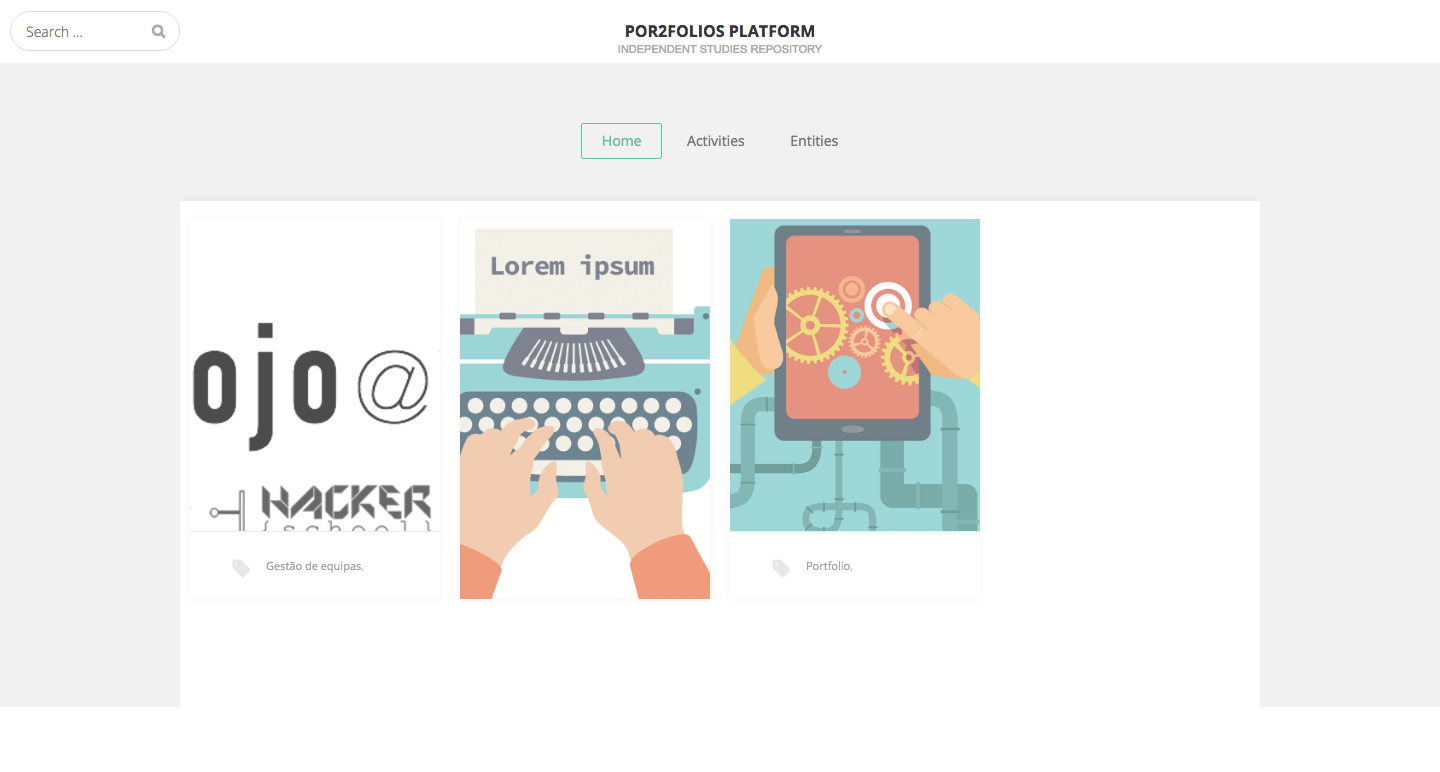
\includegraphics[width=1\linewidth]{desktop.png}
\caption{Por2folios Platform Desktop Version}
\label{fig_browser}
\end{figure}



\begin{figure}[htb]
\centering
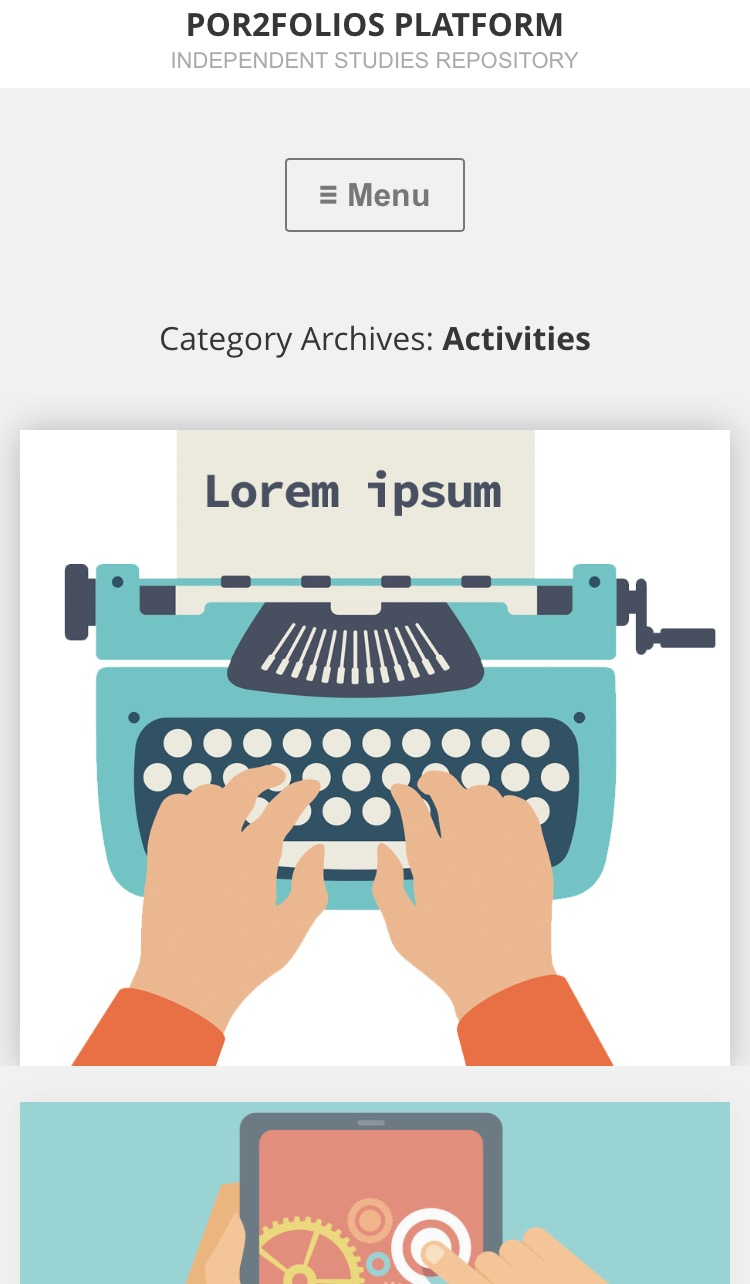
\includegraphics[width=1\linewidth]{mobile}
\caption{Por2folios Platform Mobile Version}
\label{fig_mobile}
\end{figure}


%%%%%%%%%%%%%%%%%%%%%%%%%%%%%%%%%%%%%%%%%%%%%%%%%%%%%%%%%%%%%%%%%%%%%%%%%%%%%%%%
\section{Technical Development}
For the Por2Folios platform implementation a fixed address machine was provided, hosted within the Virtual Machine of Instituto Superior Técnico. This machine was given to us, along with root accesses, with no restrictions of use whatsoever. The machine had 1Gb of Ram memory, 2Gb of virtual memory and 37Gb of storage capacity. The machine also had an out-of-date Ubunto distribution installed. To make the machine accessible we started by updating the Ubunto distribution to a more recent one (with Ubunto, the more recent the distribution, the more reliable and safer it is). Afterwards, we discussed what was the next step to take. Since we were working with a virtual machine to which we had no physical access, we decided to install a program to facilitate server management through the internet.  We used WebMin, to which access is made by the port 10000, enabling us to manage the server efficiently. This made server maintenance user friendly.

We had previously discussed what would be the best platform to develop Por2Folios. After exploring several \ac{CMS}, we concluded that WordPress was the one that better fitted our requirements. This was done before having access to the provided machine so, initially, we got the server running on a private machine. With everything installed in the private machine we launched an Alpha version of the platform, tested some functionalities, and we were able to perform some basic operations.
Having access and a port for server administration already installed in the provided machine, we then decided to migrate the WordPress from the private machine to the provided machine.
Before migrating WordPress (or any kind of \ac{CMS} actually) we had to install a HTTP server. Yet again, to facilitate the maintenance process, we used a tool which is largely documented and supported in the internet -- the Apache HTTP Server. This tool is free, runs in Windows and Unix, and 2.4 is the latest stable release. 
In order to store all the content, and to allow persistence associated with WordPress, we also had to implement a MySQL Database. Some changes were initially made to the MySql tables in order to integrate the DataBase with WordPress and, after migrating, some more changes were made to accommodate the change of domain associated with the migration to the Instituto Superior Técnico Domain.
After migrating, and to ensure security, an SSH Authentication access to the server using SSH-KEYS was implemented. This method becomes way more reliable by having the public passwords of users associated to the user account on the server. However, in order to facilitate access to future users, and to facilitate further maintenance, we continue to support the login with username and password. Both methods are currently supported.
At the moment the platform is in Beta status. Next semester we hope we'll continue to develop the platform, adding more functionalities and further enhancing the user experience.
%%%%%%%%%%%%%%%%%%%%%%%%%%%%%%%%%%%%%%%%%%%%%%%%%%%%%%%%%%%%%%%%%%%%%%%%%%%%%%%%

%%%%%%%%%%%%%%%%%%%%%%%%%%%%%%%%%%%%%%%%%%%%%%%%%%%%%%%%%%%%%%%%%%%%%%%%%%%%%%%%

\section{Future Work}

Iremos aqui falara no trabalho que deverá ser realizado no futuro ainda para mais tendo em conta que os elementos deste relatório irão todos fazer em conjunto uma evolução do projecto Por2folios.

É necessário fazer toda a documentação da plataforma, desde um manual de utilizador até a relatórios de desenvolvimento dado que esta informação será util para grupos futuros que se queiram confrontar com este projecto.

No que toca ao desenvolvimento é importante criar na plataforma uma forma de inserção standadr das actividades com entradas de tabelas predefinidas com os formatos pretendidos a serem impressos no Front-end. Esta feature será importante para o bom funcionamento da plataforma e muito provavelmente irá ser necessário aumentar a equipa para o desenvolvimento desta funcionalidade.

Por fim será necessário integrar a plataforma com uma equipa que a irá gerir e como tal será feito um trabalho na ordem dos sistemas de informação que irão testar a integração deste processo nos meios informativos da UC PPIV.

%%%%%%%%%%%%%%%%%%%%%%%%%%%%%%%%%%%%%%%%%%%%%%%%%%%%%%%%%%%%%%%%%%%%%%%%%%%%%%%%
\section{\IfLanguageName{english}{Conclusion}{Conclusão}}

No inicio desta actividades dois alunos e um aluno mais tarde partiram para o desenvolvimento de uma plataforma que iria servir como pilar informativo das várias actividades passadas das cadeiras de Portfolio Pessoal. Desta forma os novos alunos poderiam  estimar que tipo de competências transversais são possíveis de obter em cada tipo de atividade. Apesar de poucos, mas bons, conseguimos concluir a tarefa dentro de uma estimativa de horas um pouco acima das previstas no entanto ao final do dia tínhamos o trabalho cumprido.

Ainda existe muito trabalho para ser feito dentro deste projeto, começando por processar toda a informação dos documentos, tarefa essa em que seria interessante criar um classificador automático usando os mais diversos algoritmos de aprendizagem automática. Também tem de ser desenvolvida toda a infraestrutura de suporte a plataforma online, bem como a implementação da plataforma propriamente dita.

A experiência adquirida no decorrer da leitura dos relatórios foi sem duvida uma adição preciosa ao nosso desenvolvimento pessoal. O acompanhamento e disponibilidade constante do professor permitiu que a atividade se desenrolasse fluidamente e sem problemas, em que cada membro do grupo conseguiu gerir o seu tempo da melhor forma.

%%%%%%%%%%%%%%%%%%%%%%%%%%%%%%%%%%%%%%%%%%%%%%%%%%%%%%%%%%%%%%%%%%%%%%%%%%%%%%%%
% references section
\bibliographystyle{IEEEtran}
%\bibliography{PP_Report_bib}
\bibliography{Mendeley}
%%%%%%%%%%%%%%%%%%%%%%%%%%%%%%%%%%%%%%%%%%%%%%%%%%%%%%%%%%%%%%%%%%%%%%%%%%%%%%%%
% biography section
% 
\begin{IEEEbiography}[{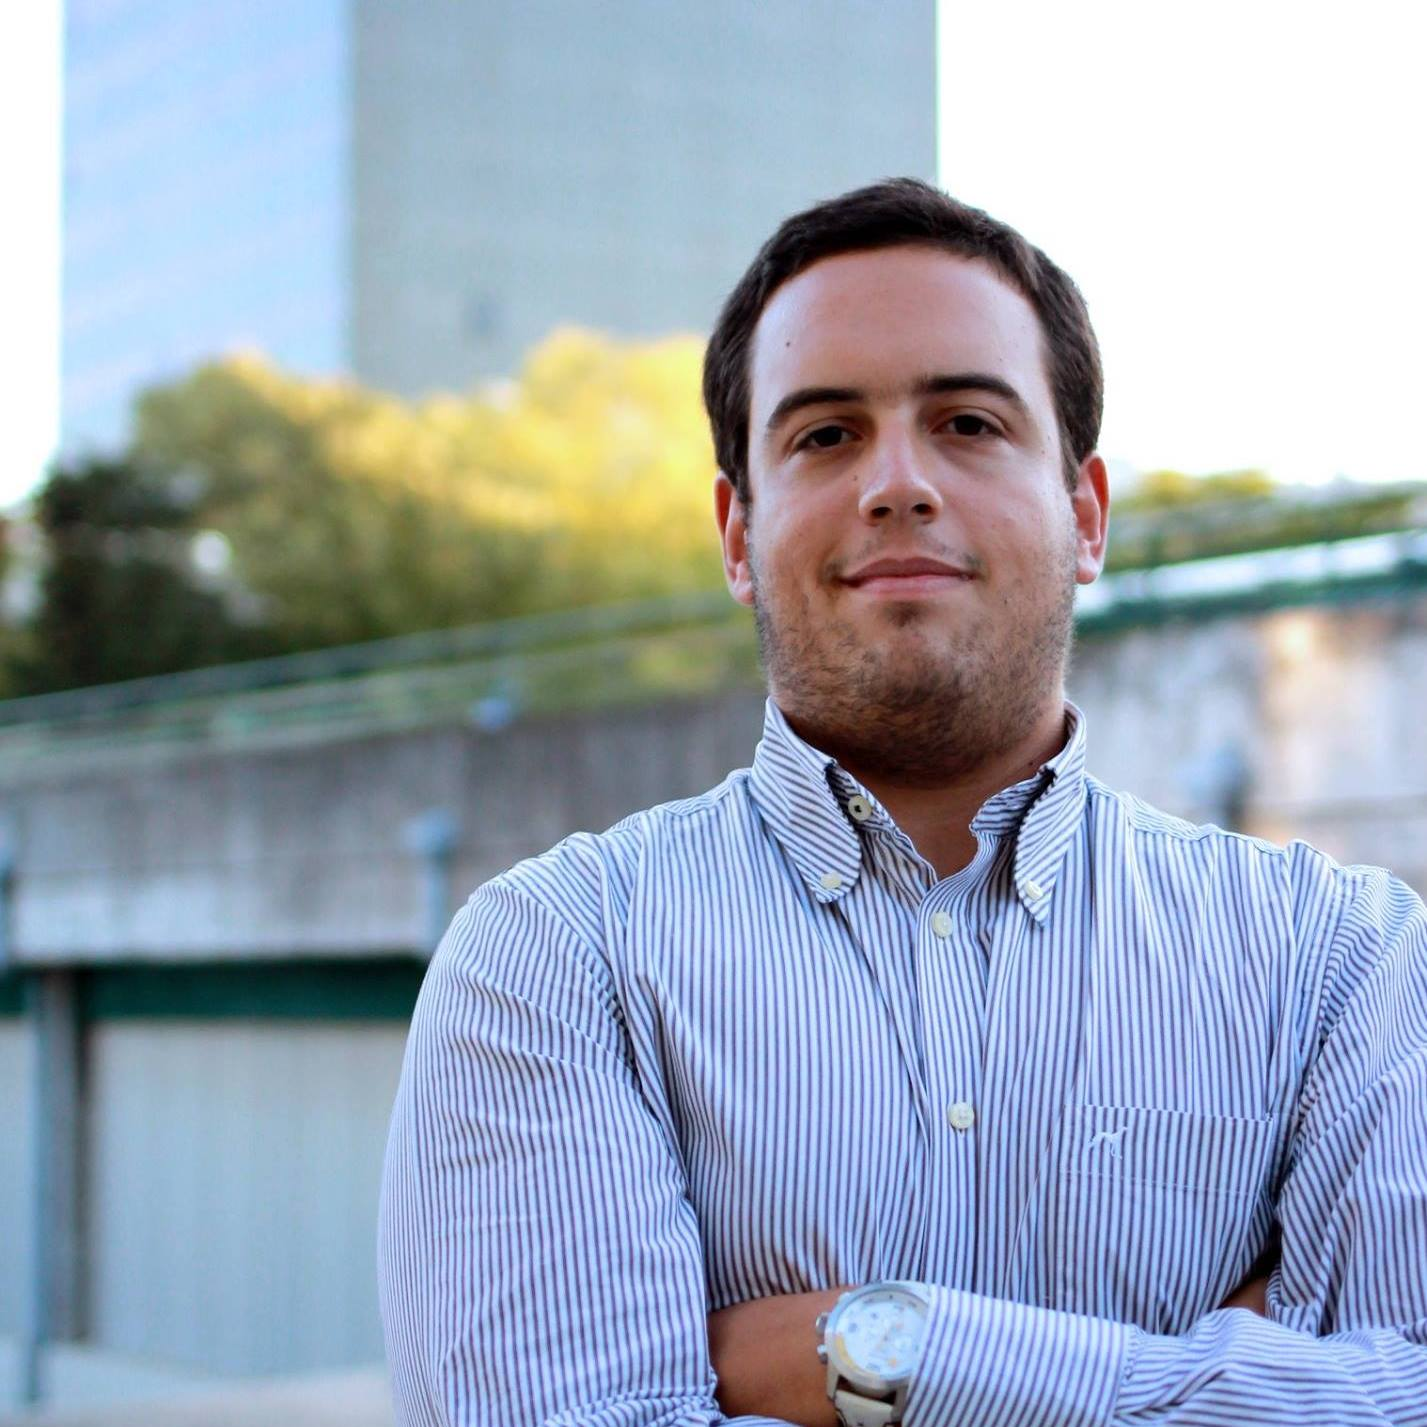
\includegraphics[width=1in,height=1.25in,clip,keepaspectratio]{bruno.png}}]{Bruno Cardoso}
Here I am. I am pursuing my Engineering studies at \ac{IST}. Starting my masters in Interaction and Visualization, and also on business systems. On my "spare" time, I am also developing a project at INESC-ID, at VIMMI.
\end{IEEEbiography}
\begin{IEEEbiography}
[{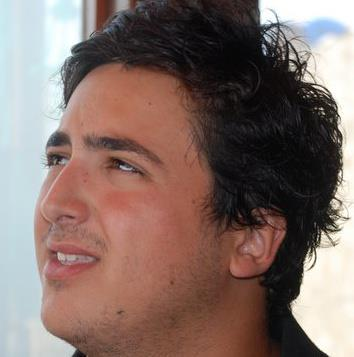
\includegraphics[width=1in,height=1.25in,clip,keepaspectratio]{francisco.png}}]{Francisco Maria Calisto}
I am pursuing my Information Systems and Computer  Engineering studies at \ac{IST}. I am also a VIMMI collaborator at INESC-ID. Currently I am working in a StartUp project called Agroop and I am Founder \& Front-end Developer of opprDev a oppr Group organisation.
\end{IEEEbiography}
\begin{IEEEbiography}
[{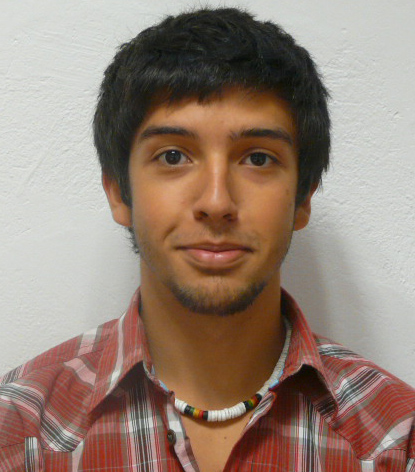
\includegraphics[width=1in,height=1.25in,clip,keepaspectratio]{nuno.png}}]{Nuno Sousa}
Here I am. I am pursuing my Engineering studies at \ac{IST}. Lorem ipsum dolor sit amet, consectetur adipiscing elit. Cras sed sapien quam. Sed dapibus est id enim facilisis, at posuere turpis adipiscing. Quisque sit amet dui dui.Lorem ipsum dolor sit amet, consectetur adipiscing elit. 
\end{IEEEbiography}



%%%%%%%%%%%%%%%%%%%%%%%%%%%%%%%%%%%%%%%%%%%%%%%%%%%%%%%%%%%%%%%%%%%%%%%%%%%%%%%%
% *** DEFINITION OF ACRONYMS ***
	\acrodef{CMS}{Content Management Systems}
	\acrodef{CPU}{Central Processing Unit}
	\acrodef{GUI}{Graphical User Interface}
	\acrodef{HTTP}{Hypertext Transfer Protocol}
	\acrodef{IST}{Instituto Superior Técnico}
	\acrodef{INESC-ID}{Instituto de Engenharia de Sistemas e Computadores - Investigação e Desenvolvimento}
	\acrodef{MEIC}{Mestrado em Engenharia Informática e de Computadores}
	\acrodef{VIMMI}{Visualization and Intelligent Multimodal Interfaces}
	\acrodef{LAN}{Local Area Network}
	\acrodef{PC}{Personal Computer}
	\acrodef{URL}{Uniform Resource Locator}
	\acrodef{VoD}{Video-on-demand}
	\acrodefplural{VoD}[VoDs]{Videos-on-demand}
	\acrodef{VoIP}{Voice over IP}
	\acrodef{WAN}{Wide Area Network}
	\acrodef{WLAN}{Wireless Local Area Network}
	\acrodef{WWAN}{Wireless Wide Area Network}
	\acrodef{WWW}{World Wide Web}

%%%%%%%%%%%%%%%%%%%%%%%%%%%%%%%%%%%%%%%%%%%%%%%%%%%%%%%%%%%%%%%%%%%%%%%%%%%%%%%%
\newpage
\onecolumn
%%%%%%%%%%%%%%%%%%%%%%%%%%%%%%%%%%%%%%%%%%%%%%%%%%%%%%%%%%%%%%%%%%%%%%%%%%%%%%%%
	
% that's all folks
\end{document}